\documentclass{standalone}
\usepackage{tikz,}

\renewcommand{\familydefault}{\sfdefault}
\usepackage{xcolor}

\usetikzlibrary{shapes.geometric, positioning}
\begin{document}
    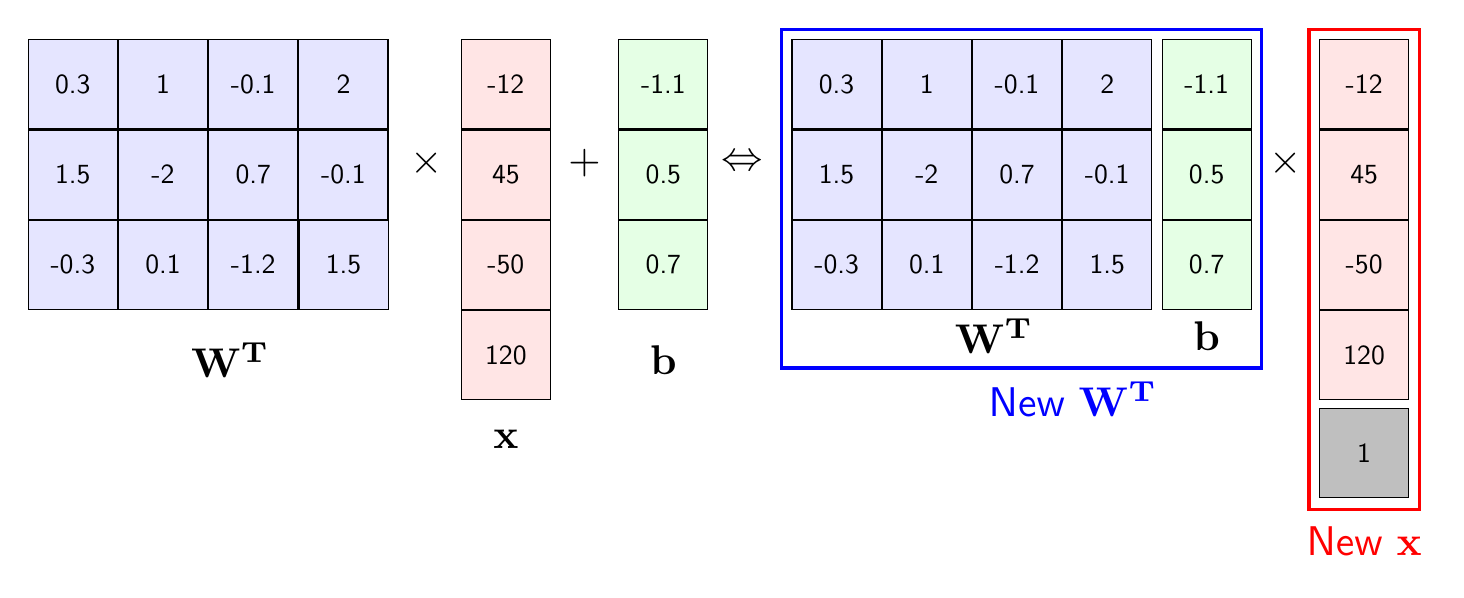
\begin{tikzpicture}[square/.style={draw, regular polygon,regular polygon sides=4, minimum width = 1.6cm}]
        % W
        \node at (0,0) [square, , fill = blue!10] (w0) {0.3};
        \node [ anchor = west, right = 0 cm of w0,square, , fill = blue!10] (w11) {1};
        \node [ anchor = west, right = 0 cm of w11,square, , fill = blue!10] (w11) {-0.1};
        \node [ anchor = west, right = 0 cm of w11,square, , fill = blue!10] (w11) {2};
            
        \node [ anchor = north, below = 0 cm of w0,square, , fill = blue!10] (w1) {1.5};
        \node [ anchor = west, right = 0 cm of w1,square, , fill = blue!10] (w11) {-2};
        \node [ anchor = west, right = 0 cm of w11,square, , fill = blue!10] (w11) {0.7};
        \node [ anchor = west, right = 0 cm of w11,square, , fill = blue!10] (w11) {-0.1};

        \node [ anchor = north, below = 0 cm of w1,square, , fill = blue!10] (w11) {-0.3};
        \node [ anchor = west, right = 0 cm of w11,square, , fill = blue!10] (w11) {0.1};
        \node [ anchor = west, right = 0 cm of w11,square, , fill = blue!10] (w11) {-1.2};
        \node [ anchor = west, right = 0 cm of w11,square, , fill = blue!10] (w11) {1.5};

        \node at (2, -3.5) [scale = 1.5] {$\mathbf{W^T}$};
        % x 
        \node at (4.5, -1) [scale = 1.5] {\bf $\times$};
        %  x
        \node at (5.5, 0) [square, fill = red!10] (w0) {-12};
        \node [anchor = north, below = 0cm of w0, square, , fill = red!10] (w1) {45};
        \node [anchor = north, below = 0cm of w1, square, , fill = red!10] (w1) {-50};
        \node [anchor = north, below = 0cm of w1, square, , fill = red!10] (w1) {120};

        \node at (5.5, -4.5) [scale = 1.5] {$\mathbf{x}$};
        % + 
        \node at (6.5, -1) [scale = 1.5] {\bf $+$};

        %  b
        \node at (7.5, 0) [square, fill = green!10] (w0) {-1.1};
        \node [anchor = north, below = 0cm of w0, square, , fill = green!10] (w1) {0.5};
        \node [anchor = north, below = 0cm of w1, square, , fill = green!10] (w1) {0.7};

        \node at (7.5, -3.5) [scale = 1.5] {$\mathbf{b}$};

        \node at (8.5, -1) [scale = 1.5] {\bf $\Leftrightarrow$};

        \begin{scope}[xshift = 9.7cm]
            % W
            \node at (0,0) [square, , fill = blue!10] (w0) {0.3};
            \node [ anchor = west, right = 0 cm of w0,square, , fill = blue!10] (w11) {1};
            \node [ anchor = west, right = 0 cm of w11,square, , fill = blue!10] (w11) {-0.1};
            \node [ anchor = west, right = 0 cm of w11,square, , fill = blue!10] (w11) {2};
                
            \node [ anchor = north, below = 0 cm of w0,square, , fill = blue!10] (w1) {1.5};
            \node [ anchor = west, right = 0 cm of w1,square, , fill = blue!10] (w11) {-2};
            \node [ anchor = west, right = 0 cm of w11,square, , fill = blue!10] (w11) {0.7};
            \node [ anchor = west, right = 0 cm of w11,square, , fill = blue!10] (w11) {-0.1};

            \node [ anchor = north, below = 0 cm of w1,square, , fill = blue!10] (w11) {-0.3};
            \node [ anchor = west, right = 0 cm of w11,square, , fill = blue!10] (w11) {0.1};
            \node [ anchor = west, right = 0 cm of w11,square, , fill = blue!10] (w11) {-1.2};
            \node [ anchor = west, right = 0 cm of w11,square, , fill = blue!10] (w11) {1.5};
            \node at (2, -3.2) [scale = 1.5] {$\mathbf{W^T}$};
            %  b
            \node at (4.7, 0) [square, fill = green!10] (w0) {-1.1};
            \node [anchor = north, below = 0cm of w0, square, , fill = green!10] (w1) {0.5};
            \node [anchor = north, below = 0cm of w1, square, , fill = green!10] (w1) {0.7};
            \node at (4.7, -3.2) [scale = 1.5] {$\mathbf{b}$};

            % x 
            \node at (5.7, -1) [scale = 1.5] {\bf $\times$};
            %  x
            \node at (6.7, 0) [square, fill = red!10] (w0) {-12};
            \node [anchor = north, below = 0cm of w0, square, , fill = red!10] (w1) {45};
            \node [anchor = north, below = 0cm of w1, square, , fill = red!10] (w1) {-50};
            \node [anchor = north, below = 0cm of w1, square, , fill = red!10] (w1) {120};
            \node [anchor = north, below = .1cm of w1, square, , fill = gray!50] (w1) {1};

            \draw [draw = blue, very thick] (-.7, -3.6) rectangle (5.4, .7);
            
            \node at (3, -4) [scale = 1.5, blue] {New $\mathbf{W^T}$};

            \draw [draw = red, very thick] (6, -5.4) rectangle (7.4, .7);
            \node at (6.7, -5.8) [scale = 1.5, red, anchor = center] {New $\mathbf{x}$};
        \end{scope}
    \end{tikzpicture}
\end{document}